\documentclass[a4paper,14pt]{article}
\usepackage[utf8]{inputenc}
\usepackage[russian]{babel}
\usepackage{geometry} % Меняем поля страницы
\geometry{left=2.5cm}% левое поле
\geometry{right=1cm}% правое поле
\geometry{top=2cm}% верхнее поле
\geometry{bottom=2cm}% нижнее поле
\setlength{\parindent}{1cm}
\parindent=1.25cm		% абзацный отступ
\linespread{1.3}     % межстрочный интервал
\tolerance=2000
\usepackage{amsmath,amssymb,graphicx,misccorr,indentfirst}
\renewcommand{\rmdefault}{cmr}
\usepackage[labelsep=period]{caption}
\usepackage{fancyhdr}
\usepackage{ragged2e}
\pagestyle{fancy}
\fancyhf{} % clear all header and footer fields
\fancyhead[C]{\thepage}
\renewcommand{\headrulewidth}{0pt}
\renewcommand{\footrulewidth}{0pt}
% redefinition of the plain style:
\fancypagestyle{plain}{%
\fancyhf{} % clear all header and footer fields
\fancyhead[C]{\thepage}
\renewcommand{\headrulewidth}{0pt}
\renewcommand{\footrulewidth}{0pt}}
\captionsetup[table]{justification=raggedright,singlelinecheck=off}
\DeclareUnicodeCharacter{2212}{-} 
\usepackage{listings}
\lstloadlanguages{Python}
\newcommand*\Laplace{\mathop{}\!\mathbin\bigtriangleup}
\newcommand*\DAlambert{\mathop{}\!\mathbin\Box}

\begin{document}
\begin{titlepage}
\begin{center}
    \large
    ФЕДЕРАЛЬНОЕ ГОСУДАРСТВЕННОЕ БЮДЖЕТНОЕ ОБРАЗОВАТЕЛЬНОЕ УЧРЕЖДЕНИЕ ВЫСШЕГО ОБРАЗОВАНИЯ «МОСКОВСКИЙ ГОСУДАРСТВЕННЫЙ УНИВЕРСИТЕТ ИМЕНИ М.В.ЛОМОНОСОВА»
     
    \textbf{Физический факультет}\\
    \vspace{4cm}
    \textsc{\Large Отчет по практическому заданию №2}\\[5mm]
    {\LARGE Основы математического моделирования.}
\end{center}
\vspace{7cm}
\null
\begin{flushright}
\normalsize студента 327 группы
\\Иванова Ивана Ивановича
\end{flushright}
\vfill
\begin{center}
\textbf{Москва - 2021}
\end{center}
\end{titlepage}


\section{Постановка задачи.}
Используя метод переменных направлений, решите краевую задачу:

\begin{equation*}
\begin{cases}
   \frac{\partial u}{\partial t} =\Laplace u + t \sin x \cos y, \ 0<x<\pi, \ 0<y<\pi, \ t>0\\
   u\bigg|_{x=0}=u\bigg|_{x=\pi}=0,\\
   \frac{\partial u}{\partial y}\bigg|_{y=0} = \frac{\partial u}{\partial y}\bigg|_{y=\pi}=0, \\
    u\bigg|_{t=0} = 0 
 \end{cases}
\end{equation*}


\section{Аналитическое решение задачи.}
Для решения поставленной краевой задачи необходимо решить следующую вспомогательную задачу Штурма-Луивилля:

\begin{equation*}
\begin{cases}
   \Laplace v + \lambda v = 0, \ 0<x<\pi, \ 0<y<\pi\\
   v\bigg|_{x=0}=v\bigg|_{x=\pi}=0,\\
   \frac{\partial v}{\partial y}\bigg|_{y=0} = \frac{\partial v}{\partial y}\bigg|_{y=\pi}=0
 \end{cases}
\end{equation*}

Решением поставленной задачи Штурма-Луивилля являются следующие собственные функции $v_{m, n}$ и собственные значения $\lambda_{m, n}$.

$$v_{m,n}=\sin nx \cos my,\ n=1,2,..., \ m = 0,1,2,...$$

$$\lambda_{m, n}=n^2+m^2$$

Разложим неоднородность $f(x,y,t)$ в уравнении теплопроводности и начальное условие $\phi(x,y)$ в ряд Фурье по системе функций $v_{n,m}$.

$$f(x, y, t) = t \sin x \cos y = t v_{1,1}(x,y)$$

$$\phi(x,y) = 0$$

\noindent Будем искать решение уравнения в следующем виде:

$$u(x,y,t)=\sum\limits_{n=1}^{\infty} \sum\limits_{m=0}^{\infty} T_{n,m}(t)v_{n,m}(x,y)$$

\noindent Подставляя в исходную задачу представления функций через ряды по системе функций $v_{n,m}$, получим следующие задачи Коши:

\begin{equation*}
\begin{cases}
   \frac{\partial T_{n,m}}{\partial t}+\lambda_{n,m}T_{n,m} = f_{n,m}\\
   T_{n,m}(0)=0
 \end{cases}
\end{equation*}


\noindent $T_{n,m}$ не равно нулю только при $n=m=1$. Решение задачи в данном случае можно записать через импульсную функцию Коши.

$$T_{1,1}=\int_0^t \tau e^{-2(t-\tau)} d\tau=\frac{1}{4}(e^{-2t}+2t-1)$$

\noindent Аналитическое решение данного уравнения теплопроводности имеет следующий вид:

$$u(x,y,t)=\frac{1}{4}(e^{-2t}+2t-1)\sin x \cos y$$

\section{Разностная схема Писмена-Рэкфорда.}
Для решения задачи воспользуемся методом переменных направлений. Для начала введем двумерную пространственную сетку и одномерную временную сетки области $\Omega = G\otimes [0,T]$.

\noindent $G=\{(x,y): 0\leq x \leq \pi,0\leq y \leq \pi\}$

\noindent $\omega_{h_x,h_y,\tau}=(x_i=ih_x, i=0,1,...,N_x; N_x h_x=\pi;\\
y_j=jh_y, y=0,1,...,N_y; N_y h_y=\pi;\\
t_k=k\tau, k=0,1,...,N_t; N_t \tau=T)$

Здесь шаг по x равен $h_x$,по y - $h_y$,а по времени - $\tau$. На введенной сетке будем рассматривать сеточную функцию  $v_{i,j}^k=u(x_i,y_j,t^k)$.

Заменим дифференциальные операторы конечноразностными: $\Laplace u \rightarrow \Lambda_1 v + \Lambda_2 v$, где 

$$\Lambda_1 v = \frac{v_{n-1,m}-2v_{n,m}+v_{n+1,m}}{h_x^2}$$

$$\Lambda_1 v = \frac{v_{n,m-1}-2v_{n,m}+v_{n,m+1}}{h_y^2}$$

$$\frac{\partial u}{\partial t} \rightarrow \frac{v^{k+1}-v^k}{\tau}$$

Согласно схеме Писмена-Рэкфорда нужно осуществлять переход со слоя k на слой k+1 в два шага, используя промежуточный (дробный) слой $k + \frac{1}{2}$. Пусть значения на слое j уже известны (на самом первом шаге значения
$u_{n,m}^0 = u(x_n, y_m, t_0)$ известны из начального условия). Перейдем на вспомогательный слой $k + \frac{1}{2}$, используя неявную схему по переменной x и явную по переменной y, то есть заменяя дифференциальный оператор $\frac{\partial^2u}{\partial x^2}$ его разностным аналогом, взятым на новом слое $k + \frac{1}{2}$, а выражение $\frac{\partial^2u}{\partial x^2}$ — разностным аналогом, взятым на слое $k$. При этом функцию $f(x, y, t)$ в правой части уравнения аппроксимируем на полуцелом слое. В результате придем к разностному уравнению:

$$\frac{v^{k+\frac{1}{2}}-v^k}{0.5\tau} = \Lambda_1 v^{k+\frac{1}{2}} + \Lambda_2 v^k + f^{k+\frac{1}{2}}$$

$$f^{k+\frac{1}{2}}=t^{k+\frac{1}{2}} \sin x \cos y$$

Переход со слоя $k+\frac{1}{2}$ на новый целый слой $k +1$ осуществим по явной схеме по направлению x и неявной по направлению y, по-прежнему аппроксимируя функцию f(x, y, t) на промежуточном полуцелом слое:

$$\frac{v^{k+1}-v^{k+\frac{1}{2}}}{0.5\tau} = \Lambda_1 v^{k+\frac{1}{2}} + \Lambda_2 v^{k+1} + f^{k+\frac{1}{2}}$$

\noindent Следовательно, получаем следующие 2 задачи:

\begin{equation*}
\begin{cases}
   \frac{v^{k+\frac{1}{2}}-v^k}{0.5\tau} = \Lambda_1 v^{k+\frac{1}{2}} + \Lambda_2 v^k + f^{k+\frac{1}{2}} \\
   v^{k+\frac{1}{2}}_{0, j} = v^{k+\frac{1}{2}}_{N_x,j}=0, \ j=0,...,N_y
 \end{cases}
\end{equation*}

\begin{equation*}
\begin{cases}
   \frac{v^{k+1}-v^{k+\frac{1}{2}}}{0.5\tau} = \Lambda_1 v^{k+\frac{1}{2}} + \Lambda_2 v^{k+1} + f^{k+\frac{1}{2}} \\
   v^{k+1}_{i, 0} = v^{k+1}_{i,1}, \ i=0,...,N_x \\
   v^{k+1}_{i,N_y-1} = v^{k+1}_{i,N_y}, \ i=0,...,N_x
 \end{cases}
\end{equation*}

В последней задаче граничные условия Неймана были аппроксимированы разностным оператором с первым порядком аппроксимации по координате $x$. Сама же схема переменных направлений имеет второй порядок аппроксимации по времени и координатам.

\noindent Используя явный вид операторов, получим задачи: $t^{m} \rightarrow t^{m+ \frac{1}{2}}$.

$$\frac{0.5 \tau}{h_x^2} v_{i-1,j}^{k+\frac{1}{2}} - (1+\frac{\tau}{h_x^2})v_{i,j}^{k+\frac{1}{2}} + \frac{0.5 \tau}{h_x^2} v_{i+1,j}^{k+\frac{1}{2}} = -F_{i,j}^{k+\frac{1}{2}}$$

$$F_{i,j}^{k+\frac{1}{2}} = \frac{0.5 \tau}{h_y^2} (v_{i,j-1}^{k}+v_{i,j+1}^{k})+(1-\frac{\tau}{h_y^2})v_{i,j}^{k} + 0.5 \tau f^{k+\frac{1}{2}}_{i,j}$$

$$v^{k+\frac{1}{2}}_{0, j} = v^{k+\frac{1}{2}}_{N_x,j}=0, \ j=0,...,N_y$$


Это СЛАУ относительно переменных $v_{i+1,j}^{k+\frac{1}{2}}, \ v_{i,j}^{k+\frac{1}{2}}, \ v_{i-1,j}^{k+\frac{1}{2}}$. Для нахождения решения но новом слое, необходимо перебрать все j, и при каждом j решаем систему уравнений методом прогонки. $i = 0,...,N_x, \ j=0,...,N_y$.

Рассмотрю переход на следующий слой: $t^{m+ \frac{1}{2}} \rightarrow t^{m+1}$.

$$\frac{0.5 \tau}{h_y^2} v_{i,j-1}^{k+1} - (1+\frac{\tau}{h_y^2})v_{i,j}^{k+1} + \frac{0.5 \tau}{h_y^2} v_{i,j+1}^{k+1} = -F_{i,j}^{k+1}$$

$$F_{i,j}^{k+1} = \frac{0.5 \tau}{h_x^2} (v_{i-1,j}^{k+\frac{1}{2}}+v_{i+1,j}^{k+\frac{1}{2}})+(1-\frac{\tau}{h_x^2})v_{i,j}^{k+\frac{1}{2}} + 0.5 \tau f^{k+\frac{1}{2}}_{i,j}$$

$$ v^{k+1}_{i, 0} = v^{k+1}_{i,1}, \ v^{k+1}_{i,N_y-1} = v^{k+1}_{i,N_y}, \ i=0,...,N_x$$

Это СЛАУ относительно переменных $v_{i,j+1}^{k+1}, \ v_{i,j}^{k+1}, \ v_{i,j-1}^{k+1}$. Для нахождения решения но новом слое, необходимо перебрать все i, и при каждом i решаем систему уравнений методом прогонки. $i = 0,...,N_x, \ j=0,...,N_y$.

Важно отметить, что разностная схема Писмена-Рэкфорда является экономичной разностной схемой, т.е. она является безусловно устойчивой и требует при переходе со слоя на слой числаарифметических операций, пропорционального числу узлов сетки.

\section{Метод прогонки.}
Необходимо решить следующую систему уравнений:

$$A y_{m+1} - C y_m + B y_{m-1}=F_m$$

$$y_0 = k_1 y_1 + \mu_1, \ y_M = k_2 y_{M-1} + \mu_2$$

Метод прогонки годится, если $B_m > A_m + C_m, 0 \leq k_{1,2} \leq 1$, либо
$B_m \geq A_m + C_m, 0  \leq  k_{1,2} < 1$. Для выписанной выше СЛАУ это условие выполняется.

Ищем решение в виде: $y_m = d_{m+1}y_{m+1}+\sigma_{m+1}$. Подставляя решения в исходное уравнение, получаем рекуррентные формулы для определения прогоночных коэффициентов:

$$d_{m+1} = \frac{C_m}{B_m-A_m d_m}, \ m=0,...,M-1$$

$$\sigma_{m+1}=\frac{F_m-A_m \sigma_m}{A_m d_m - B_m}, \ m=0,...,M-1$$

\noindent Из того, что $y_0 = k_1, \ y_1 + \mu_1$ находим, что $d_1 = k_1, \sigma_1 = \mu_1$.

Из рекуррентных формул находим (прямая прогонка) $d_M, \ \sigma_M$. Отсюда находим, что: $$y_M= \frac{k_2 \sigma_M + \mu_2}{1-k_2 d_M}$$

Далее производим обратную прогонку: $y_m = d_{m+1}y_{m+1}+\sigma_{m+1}$ и находим все $y_m$ решения линейной системы уравнений.

Этот метод уникален тем, что арифметическая сложность данного алгоритма пропорциональна количеству неизвестных $O(N)$, в то время, как арифметическая сложность метода Гаусса пропорциональна квадрату количества неизвестных $O(N^2)$.

Рассмотрю два типа начальных условий: 1) Условия Дирихле

\noindent $y_0 = 0, \ y_M = 0$, из этого следует, что $d_1 = 0, \ \sigma_1 = 0$. 

2) Условия Неймана

\noindent Воспользуемся приближением производной с помощью разностного оператора:

$$\frac{y_1 - y_0}{h} = 0, \ \frac{y_M - y_{M-1}}{h} = 0$$

\noindent Из вида граничных условий имеем, что $d_1 = d_M = 1, \ \sigma_1 = \sigma_M = 0$.

\section{Проверка сходимости по спектральному критерию Неймана.}
Пусть в начальные условия внесена некоторая ошибка: $\phi \rightarrow \phi + \delta \phi$. Тогда в решении тоже появится появится ошибка: $u \rightarrow u + \delta u$. Раскладываем ошибку в ряд Фурье и исследуем поведение каждой отдельной гармоники при переходе с одного слоя на последующий. Для поставленной задачи имеем следующее уравнение для ошибки:

$$\delta u_t = \Laplace \delta u$$

Для этого уравнения напишем разностную схему Писмена-Рэкфорда. Обозначу ошибку следующим образом: $\delta u \rightarrow v$

$$\frac{0.5 \tau}{h_x^2} (v_{i-1,j}^{k+\frac{1}{2}} + v_{i+1,j}^{k+\frac{1}{2}}) - (1+\frac{\tau}{h_x^2})v_{i,j}^{k+\frac{1}{2}} + \frac{0.5 \tau}{h_y^2} (v_{i,j-1}^{k}+v_{i,j+1}^{k})+(1-\frac{\tau}{h_y^2})v_{i,j}^{k}=0$$

$$\frac{0.5 \tau}{h_y^2} (v_{i,j-1}^{k+1} + v_{i,j+1}^{k+1})- (1+\frac{\tau}{h_y^2})v_{i,j}^{k+1} + \frac{0.5 \tau}{h_x^2} (v_{i-1,j}^{k+\frac{1}{2}}+v_{i+1,j}^{k+\frac{1}{2}})+(1-\frac{\tau}{h_x^2})v_{i,j}^{k+\frac{1}{2}} = 0$$

\noindent Подставляем в первое разностное уравнение $v_{i,j}^k = \lambda^{k}_1 \exp(I(\omega_1 i + \omega_2 j))$, во второе $v_{i,j}^k = \lambda^{k}_2 \exp(I(\omega_1 i + \omega_2 j))$.

После некоторых преобразований получаем следующие уравнения:

$$\frac{0.5 \tau}{h_x^2} \lambda^{0.5}_1(e^{I \omega_1}+e^{-I \omega_1})-(1+\frac{\tau}{h_x^2})\lambda^{0.5}_1+\frac{0.5 \tau}{h_y^2} (e^{I \omega_2}+e^{-I \omega_2})+(1-\frac{\tau}{h_y^2})=0$$

$$\frac{0.5 \tau}{h_y^2} \lambda^{0.5}_2(e^{I \omega_2}+e^{-I \omega_2})-(1+\frac{\tau}{h_y^2})\lambda^{0.5}_2+\frac{0.5 \tau}{h_x^2} (e^{I \omega_1}+e^{-I \omega_1})+(1-\frac{\tau}{h_x^2})=0$$

В итоге получаем следующие выражения для множителей роста:

$$\lambda_1^{0.5} = \frac{1-\frac{2\tau}{h_y^2} \sin^2(\frac{\omega_2}{2})}{1+\frac{2\tau}{h_x^2} \sin^2(\frac{\omega_1}{2})}$$

$$\lambda_2^{0.5} = \frac{1-\frac{2\tau}{h_x^2} \sin^2(\frac{\omega_1}{2})}{1+\frac{2\tau}{h_y^2} \sin^2(\frac{\omega_2}{2})}$$

\noindent Из вида выражений для множителей роста видно, что $\lambda_1$ и $\lambda_2$ меньше единицы $\forall \ h_x, \ h_y, \ \tau, \ \omega_1, \ \omega_2$. Из этих соотношений получаем, что $|\lambda_1 \lambda_2| < 1$ $\forall \ h_x, \ h_y, \ \tau, \ \omega_1, \ \omega_2$. Это означает, что необходимое условие устойчивости (спектральный критерий Неймана) разностной схемы выполнено. Схема является безусловно устойчивой.

\section{Порядок аппроксимации разностной схемы.}
Вычислим порядок аппроксимации (невязку) для этого шаблона. Для этого выберем некоторую функцию $u(x,y,t)$ непрерывных переменных. Подставляем эту функцию в разностную схему, выбираем точку $(x_i, y_j, t^{k+0.5})$. Разложим функции в ряд Тейлора в этой точке.

Для краткости обозначу функцию $u(x_i, y_j, t^{k+0.5})=u$

$$u(x_{i \pm 1}, y_j, t^{k}) = u + (-\frac{\partial}{\partial t}\frac{\tau}{2}\pm \frac{\partial}{\partial x}h_x)u+
\frac{1}{2}(-\frac{\partial}{\partial t}\frac{\tau}{2} \pm \frac{\partial }{\partial x}h_x)^2 u + 
\frac{1}{6}(-\frac{\partial}{\partial t}\frac{\tau}{2} \pm \frac{\partial}{\partial x}h_x)^3 u +
\frac{1}{24}(-\frac{\partial}{\partial t}\frac{\tau}{2} \pm \frac{\partial}{\partial x}h_x)^4 u +...$$

$$u(x_i, y_{j \pm 1}, t^{k + 1}) = u + (\frac{\partial}{\partial t}\frac{\tau}{2}\pm \frac{\partial}{\partial y}h_y)u+
\frac{1}{2}(\frac{\partial}{\partial t}\frac{\tau}{2} \pm \frac{\partial }{\partial y}h_y)^2 u + 
\frac{1}{6}(\frac{\partial}{\partial t}\frac{\tau}{2} \pm \frac{\partial}{\partial y}h_y)^3 u +
\frac{1}{24}(\frac{\partial}{\partial t}\frac{\tau}{2} \pm \frac{\partial}{\partial y}h_y)^4 u +...$$

$$u(x_i, y_j, t^{k}) = u - \frac{\partial u}{\partial t}\frac{\tau}{2} + \frac{1}{2} \frac{\partial^2 u}{\partial t^2}\frac{\tau^2}{4} -
\frac{1}{6} \frac{\partial^3 u}{\partial t^3}\frac{\tau^3}{8} +
\frac{1}{24} \frac{\partial^4 u}{\partial t^4}\frac{\tau^4}{16} + ...$$

$$u(x_i, y_j, t^{k+1}) = u + \frac{\partial u}{\partial t}\frac{\tau}{2} + \frac{1}{2} \frac{\partial^2 u}{\partial t^2}\frac{\tau^2}{4} +
\frac{1}{6} \frac{\partial^3 u}{\partial t^3}\frac{\tau^3}{8} +
\frac{1}{24} \frac{\partial^4 u}{\partial t^4}\frac{\tau^4}{16} + ...$$

$$u(x_{i \pm 1} , y_j, t^{k+0.5}) = u \pm \frac{\partial u}{\partial x} h_x + \frac{1}{2} \frac{\partial^2 u}{\partial x^2}h_x^2 \pm
\frac{1}{6} \frac{\partial^3 u}{\partial x^3}h_x^3 +
\frac{1}{24} \frac{\partial^4 u}{\partial x^4}h_x^4 + ...$$

$$u(x_i, y_{j \pm 1}, t^{k+0.5}) = u \pm \frac{\partial u}{\partial y} h_y + \frac{1}{2} \frac{\partial^2 u}{\partial y^2}h_y^2 \pm
\frac{1}{6} \frac{\partial^3 u}{\partial y^3}h_y^3 +
\frac{1}{24} \frac{\partial^4 u}{\partial y^4}h_y^4 + ...$$

\noindent подставляем найденные выражения в разностную схему:

$$\frac{\partial^2 u}{\partial x^2} + \frac{h_x^2}{12} \frac{\partial^4 u}{\partial x^4} + \frac{\partial^2 u}{\partial y^2}- \frac{1}{2} \frac{\partial^3 u}{\partial t \partial y^2} \tau + \frac{1}{8}\frac{\partial^4 u}{\partial t^2 \partial y^2} \tau^2 + \frac{h_y^2}{12} \frac{\partial^4 u}{\partial y^4} - \frac{\partial u}{\partial t}+ \frac{1}{2}\frac{\partial^2 u}{\partial t^2}\frac{\tau}{2}- \frac{1}{6}\frac{\partial^3 u}{\partial t^3}\frac{\tau^2}{4}+\frac{1}{24}\frac{\partial^4 u}{\partial t^4}\frac{\tau^3}{8}=0$$

$$\frac{\partial^2 u}{\partial x^2} + \frac{h_x^2}{12} \frac{\partial^4 u}{\partial x^4} + \frac{\partial^2 u}{\partial y^2}+ \frac{1}{2} \frac{\partial^3 u}{\partial t \partial y^2} \tau + \frac{1}{8}\frac{\partial^4 u}{\partial t^2 \partial y^2} \tau^2 + \frac{h_y^2}{12} \frac{\partial^4 u}{\partial y^4} - \frac{\partial u}{\partial t} - \frac{1}{2}\frac{\partial^2 u}{\partial t^2}\frac{\tau}{2}- \frac{1}{6}\frac{\partial^3 u}{\partial t^3}\frac{\tau^2}{4}-\frac{1}{24}\frac{\partial^4 u}{\partial t^4}\frac{\tau^3}{8}=0$$

\noindent Найдём невязку, вычитая из каждого уравнения точный дифференциальный оператор уравнения теплопроводности

$$\frac{h_x^2}{12} \frac{\partial^4 u}{\partial x^4} - \frac{1}{2} \frac{\partial^3 u}{\partial t \partial y^2} \tau + \frac{1}{8}\frac{\partial^4 u}{\partial t^2 \partial y^2} \tau^2 + \frac{h_y^2}{12} \frac{\partial^4 u}{\partial y^4} + \frac{1}{2}\frac{\partial^2 u}{\partial t^2}\frac{\tau}{2}- \frac{1}{6}\frac{\partial^3 u}{\partial t^3}\frac{\tau^2}{4}+\frac{1}{24}\frac{\partial^4 u}{\partial t^4}\frac{\tau^3}{8}$$

$$\frac{h_x^2}{12} \frac{\partial^4 u}{\partial x^4} + \frac{1}{2} \frac{\partial^3 u}{\partial t \partial y^2} \tau + \frac{1}{8}\frac{\partial^4 u}{\partial t^2 \partial y^2} \tau^2 + \frac{h_y^2}{12} \frac{\partial^4 u}{\partial y^4} - \frac{1}{2}\frac{\partial^2 u}{\partial t^2}\frac{\tau}{2}- \frac{1}{6}\frac{\partial^3 u}{\partial t^3}\frac{\tau^2}{4}-\frac{1}{24}\frac{\partial^4 u}{\partial t^4}\frac{\tau^3}{8}$$

Складывая эти два выражения, получим порядок аппроксимации разностной схемы Писмена-Рэкфорда.

$$\frac{h_x^2}{6} \frac{\partial^4 u}{\partial x^4} + \frac{h_y^2}{6} \frac{\partial^4 u}{\partial y^4}+\frac{1}{4}\frac{\partial^4 u}{\partial t^2 \partial y^2} \tau^2 - \frac{1}{3}\frac{\partial^3 u}{\partial t^3}\frac{\tau^2}{4}= O(h_x^2+h_y^2+\tau^2)$$

Таким образом, разностная схема Писмена-Рэкфорда имеет второй порядок аппроксимации по пространственным координатам и времени. Так как данная схема обладает безусловной устойчивостью, то тогда она сходится со вторым порядком по пространственным координатам и времени.

\section{Результаты.}
В результате выполнения программы получены следующие графики:

\begin{figure}[h!]
\centering
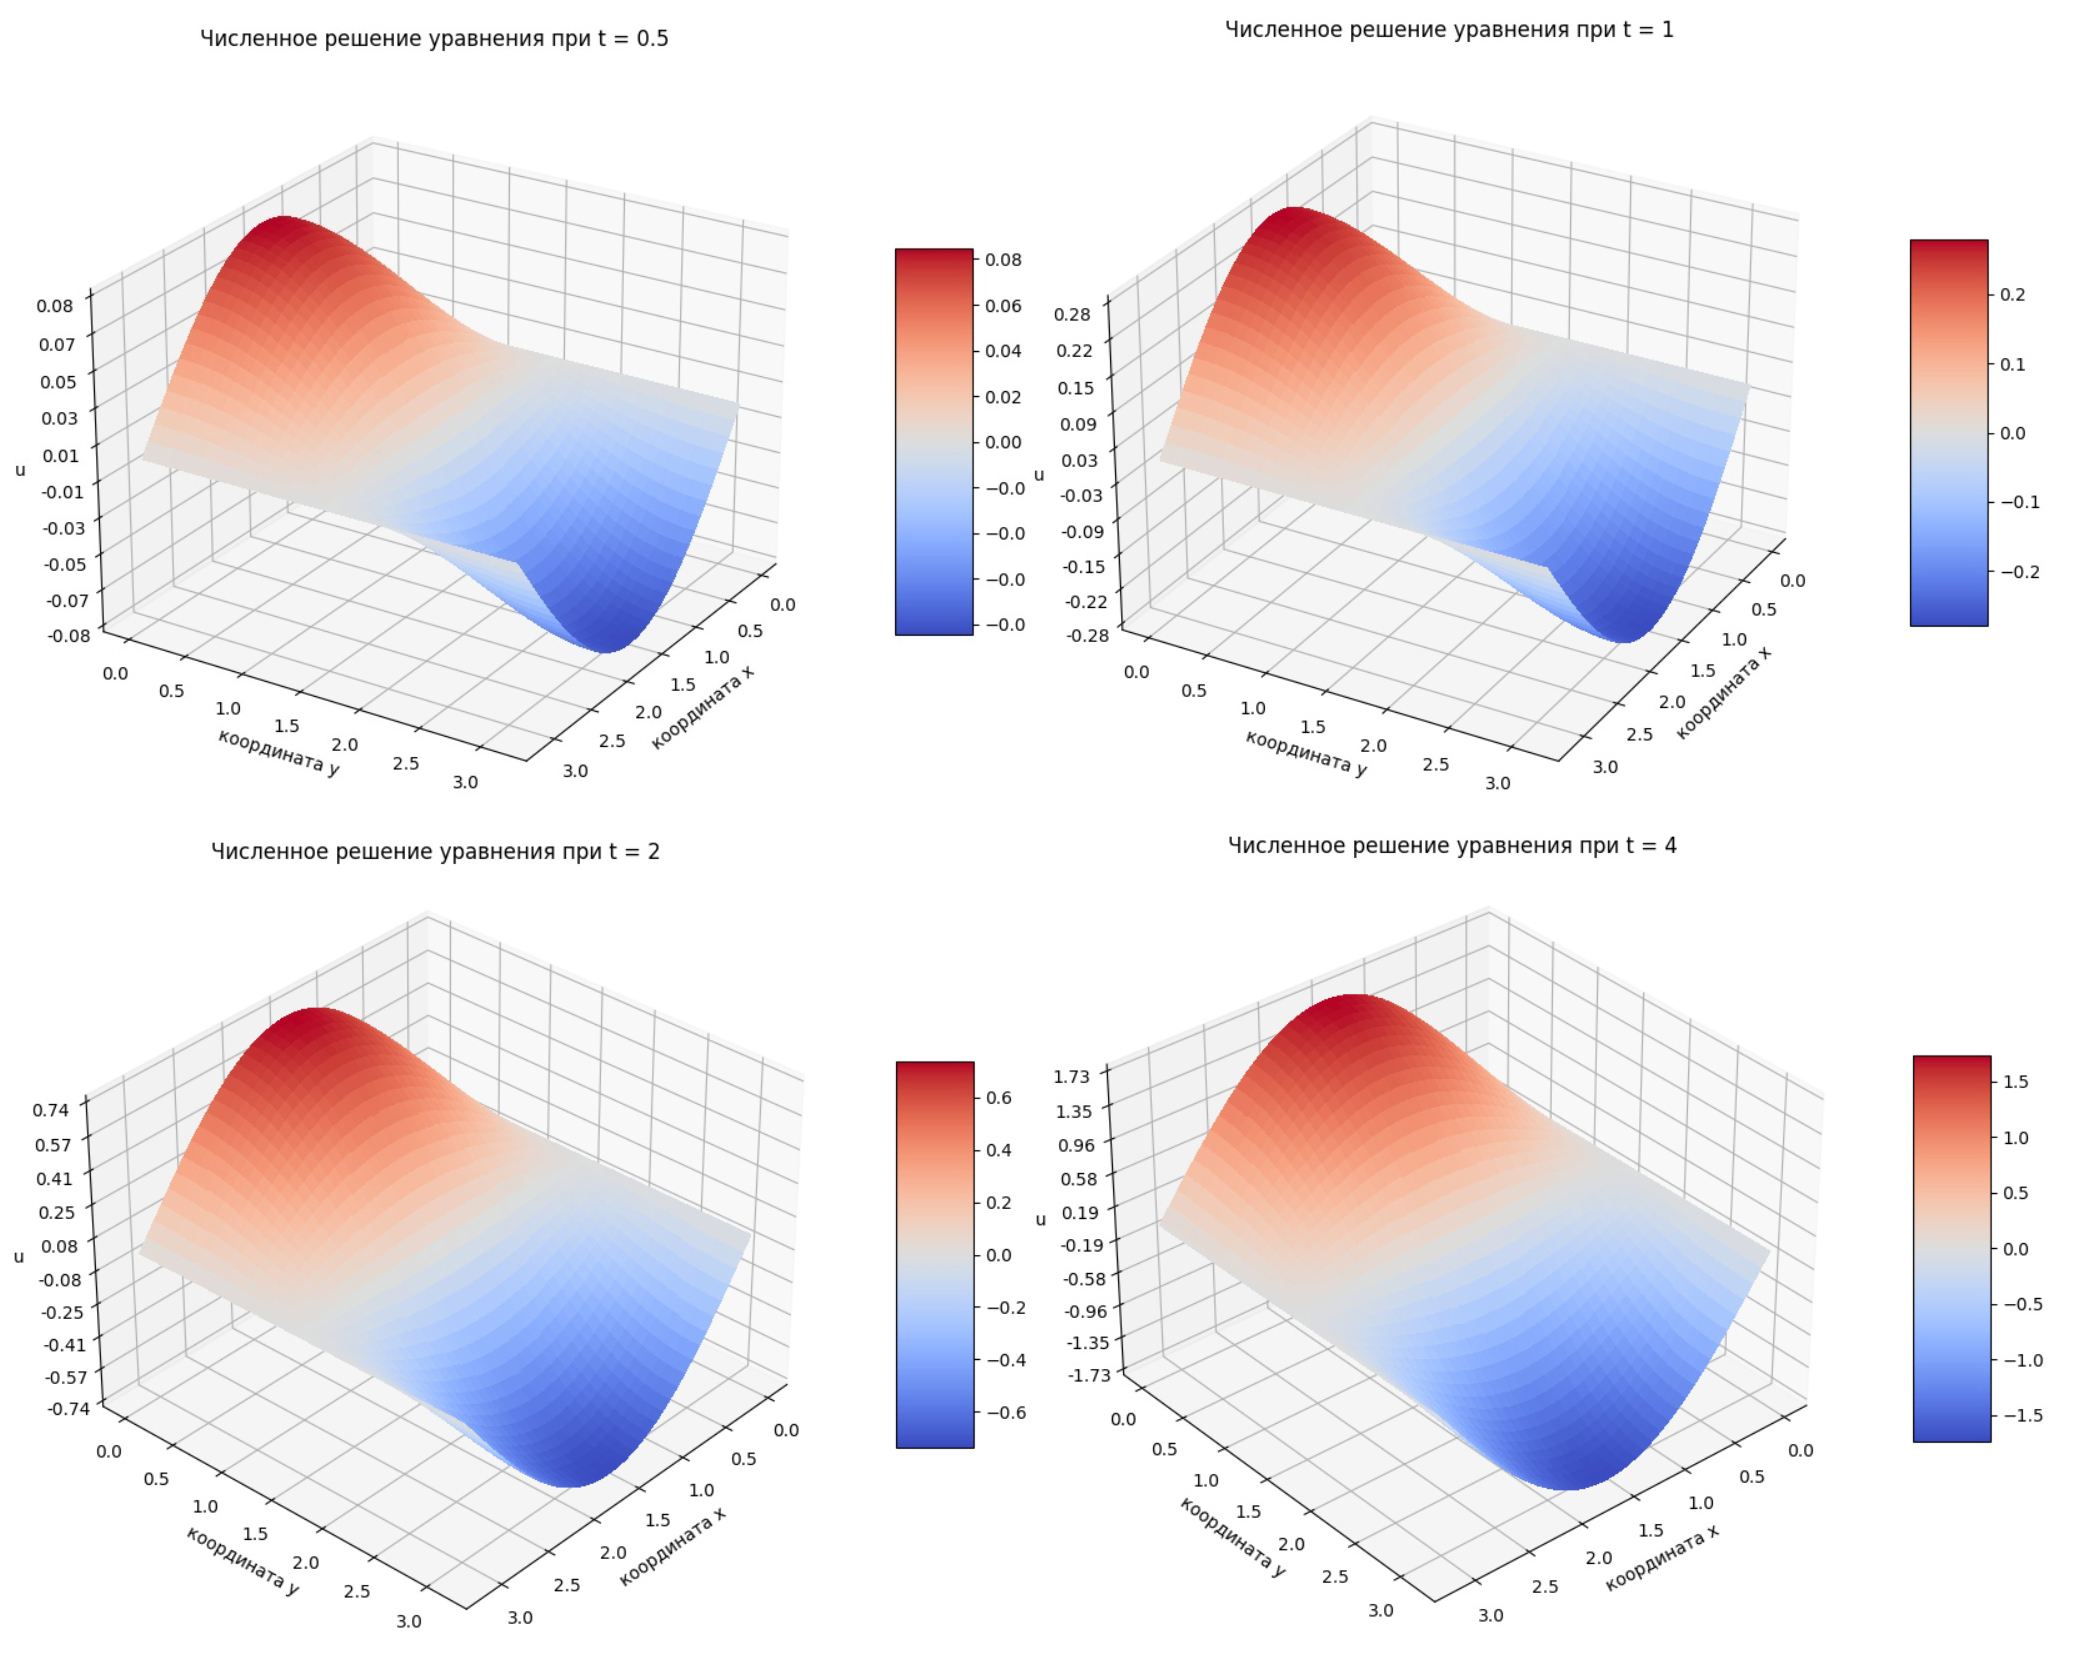
\includegraphics[scale=0.25]{решение.jpg}
\caption{\label{pic1} Численное решение уравнения при разных значениях t}
\end{figure}

Также численное решение сравнили с точным на разных сетках. Из рисунков \ref{pic2}, \ref{pic3} видно, что численное решение приближается к точному при уменьшении шага сетки, что соответствует теоретическим выкладкам. Стоит ещё раз отметить, что разностная схема Писмена-Рэкфорда имеет порядок второй аппроксимации, а граничные условия Неймана по оси $y$ аппроксимировались односторонней разностью, то порядок точности всей схемы не второй, а первый. Это можно увидеть и по графикам расчета при разных шагах сетки.

\begin{figure}[h!]
\centering
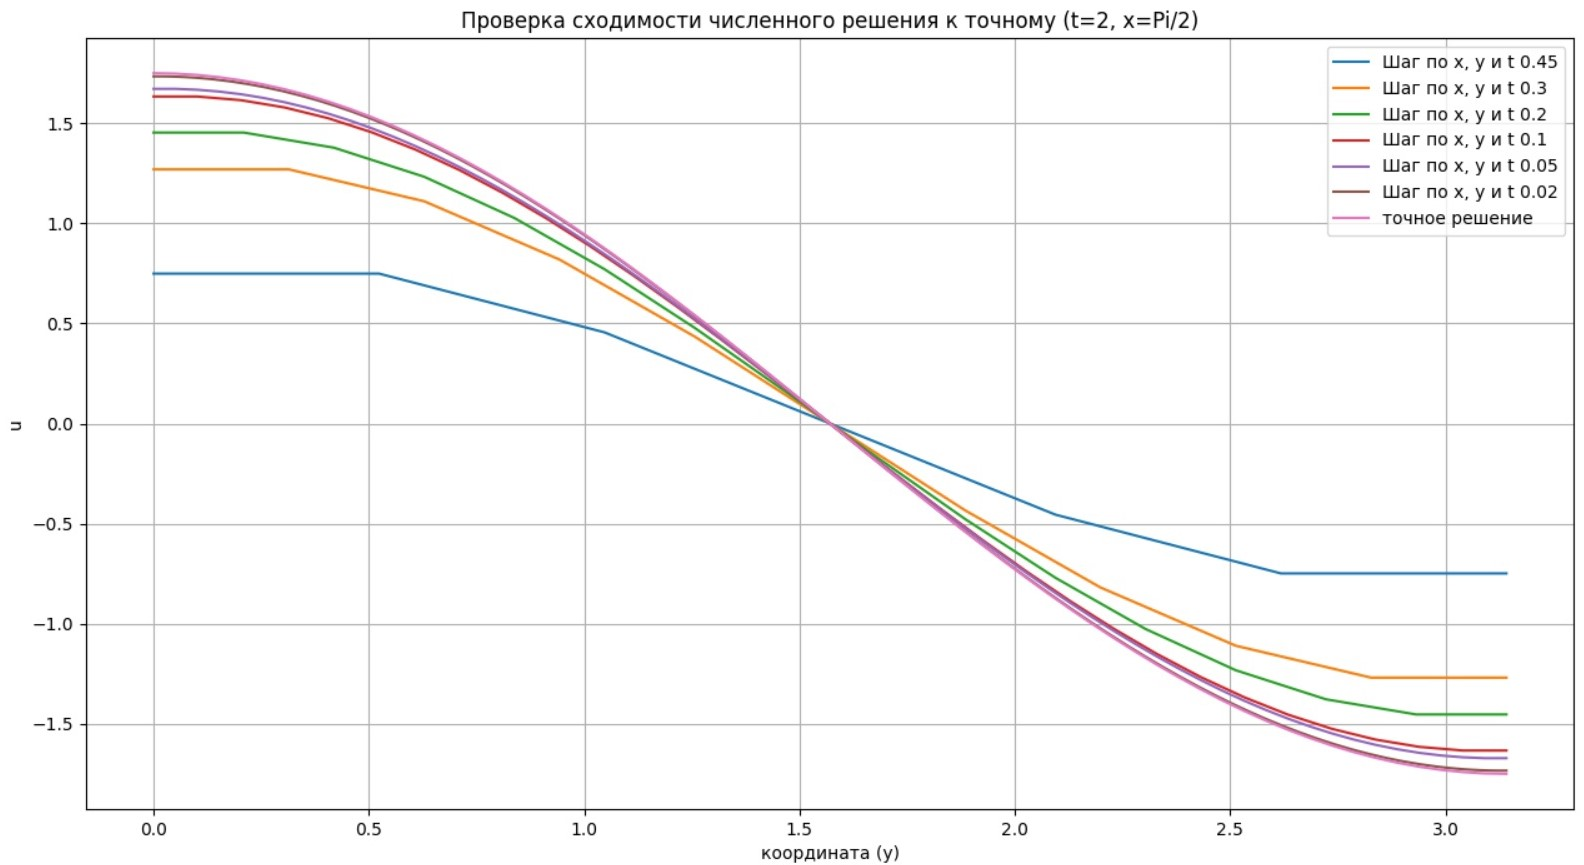
\includegraphics[scale=0.4]{проверка 1.jpg}
\caption{\label{pic2}}
\end{figure} 

\begin{figure}[h!]
\centering
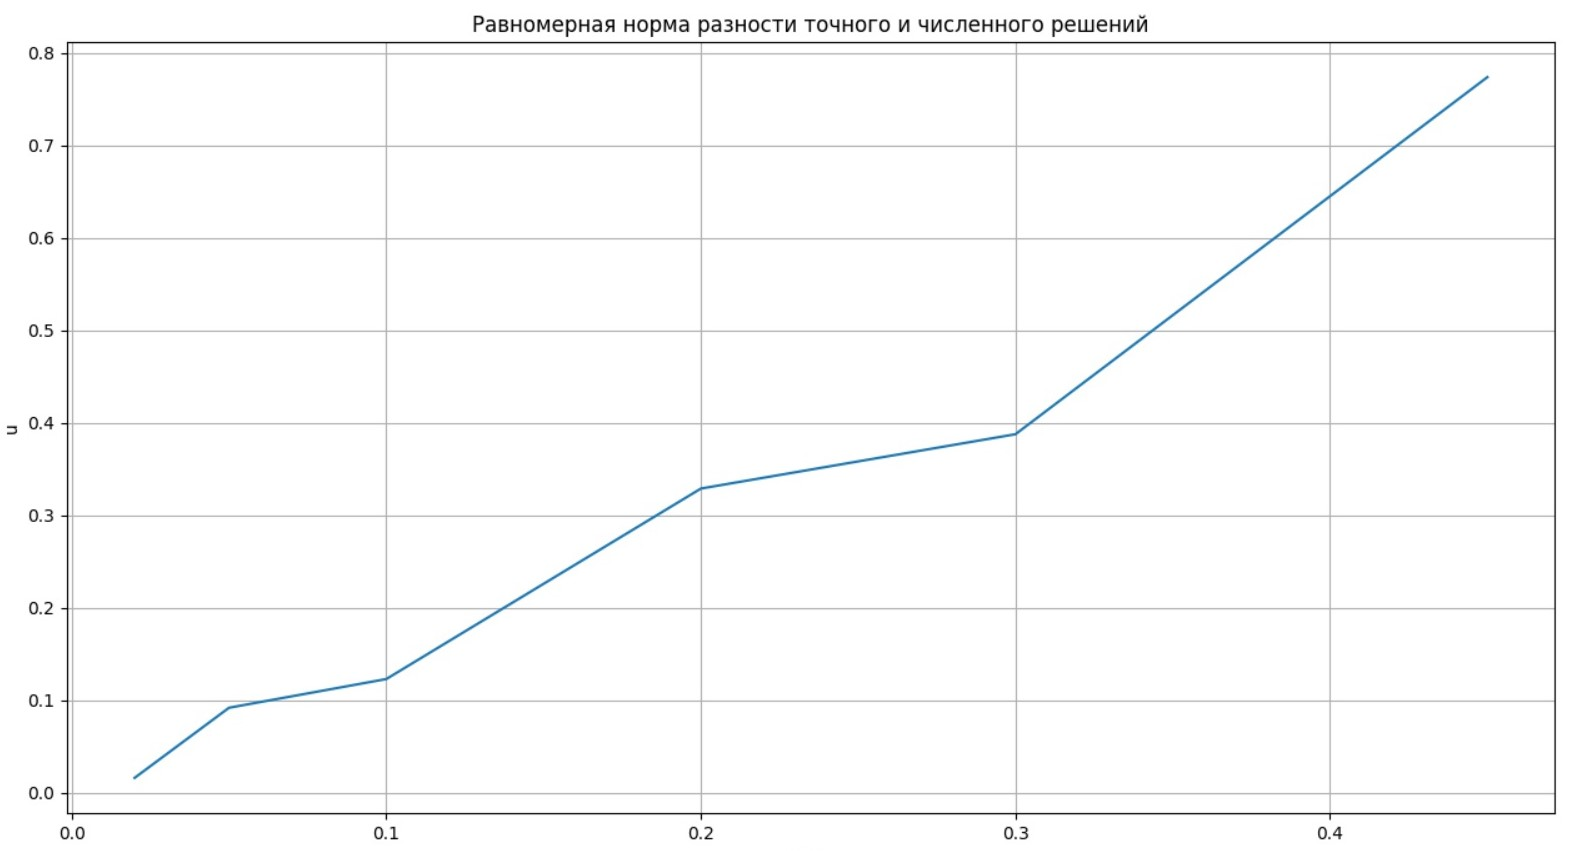
\includegraphics[scale=0.4]{проверка 2.jpg}
\caption{\label{pic3}}
\end{figure} 

На рисунках \ref{pic4}, \ref{pic5}, \ref{pic6} продемонстрирована проверка граничных и начальных условий численного рещения.

\begin{figure}[h!]
\centering
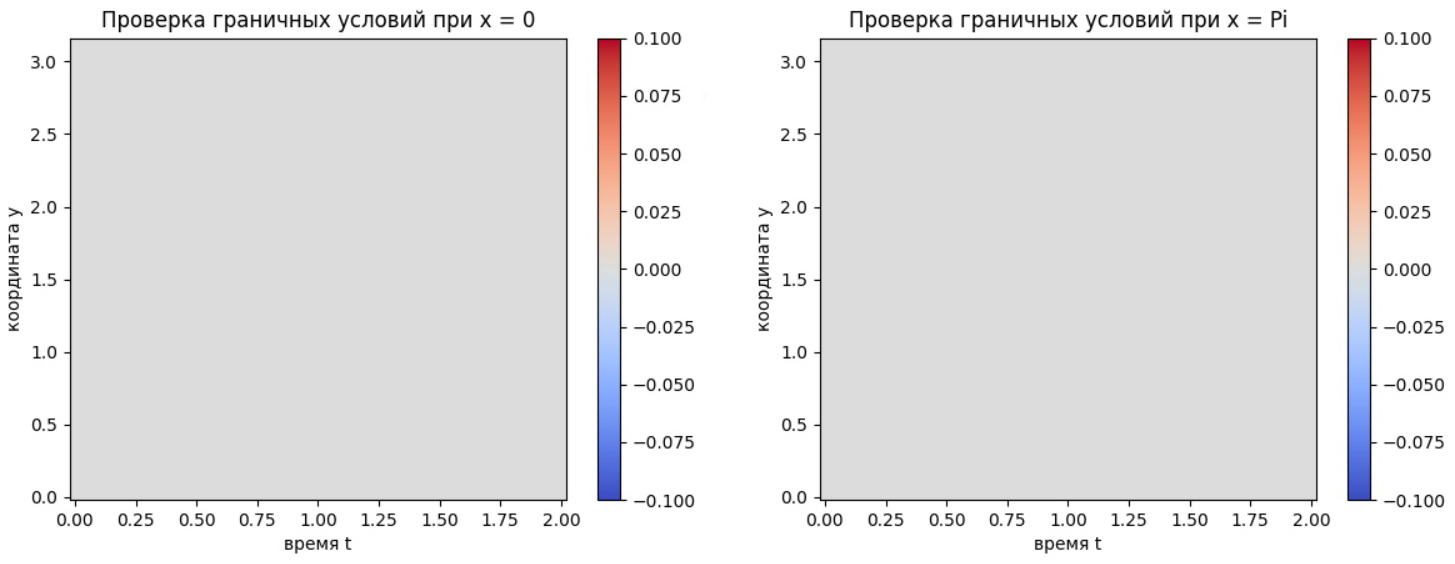
\includegraphics[scale=0.3]{гу x.jpg}
\caption{\label{pic4}}
\end{figure} 

\begin{figure}[h!]
\centering
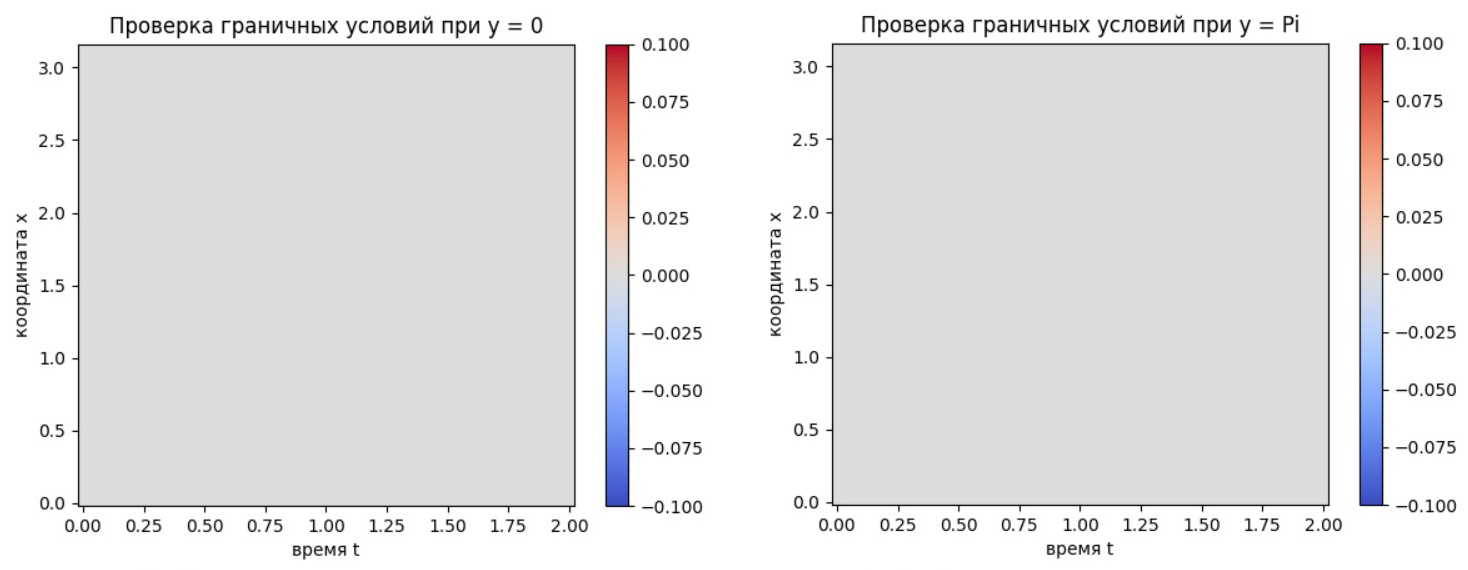
\includegraphics[scale=0.3]{гу y.jpg}
\caption{\label{pic5}}
\end{figure} 

\begin{figure}[h!]
\centering
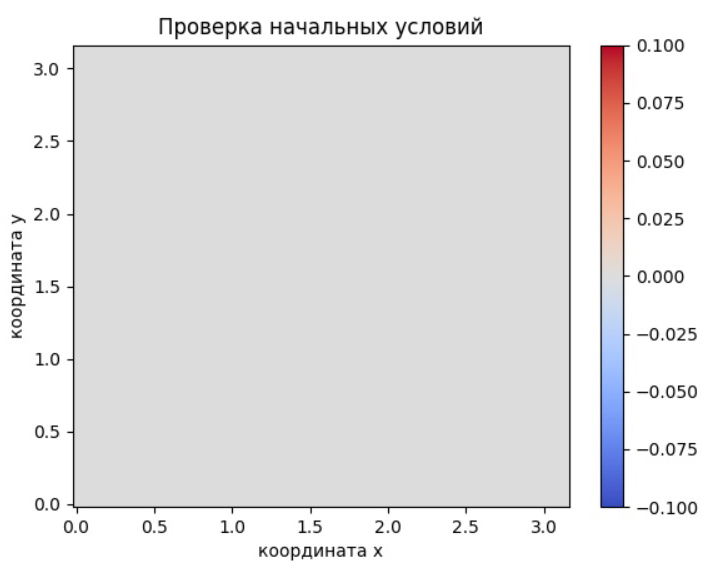
\includegraphics[scale=0.3]{ну.jpg}
\caption{\label{pic6}}
\end{figure} 

\end{document}
